\section{Software Design}
  Following the design of the mechanical and electrical aspects of the rover was that of the software as hosted by the RCE as well as for user control and interaction. The section covers the design process undertaken before and during the development of the software for all aspects of the project. The software design and development processes were highly iterative as many of the design choices had to be made after realisation of the technology capabilities and conversely, many of the technology choices were made based on what was required on a more functional and detailed level at design time. The two processes are separated as far as possible in this report for a friendlier structure, however, much of the design detail is included in the development sections.
  
  The design stage initiated with an overview of the requirements, a plan of the designed structures of each of the subsystems as categorised in the overview and descriptions of the technologies that were chosen for development.
  
  \subsection{Systems Overview in Context}
    An attempt was made to mimic the communications and software structures and patterns used for MSL (and other similar missions) and as such, the software system for this project resembles the three component structure consisting of a system on the rover, the software employed for the collection of relay satellites and ground-based DSN hardware, and the client front-end software as used by the MSL team. Figure~\ref{fig:specs-functionalBreakdown} already highlights the basic breakdown of the software systems. As discussed in Section~\ref{subsubsec:rover-equivalence}, the three major software subsystems by name included the Rover Compute Element (RCE) and the Robot Sequencing and Visualisation Program (RSVP) divided further into the Server and the Client.
    
    The RCE was hosted by the computational hardware on the rover (the Intel Edison board, here-onwards referred to as the RCE board) and required control of hardware, sensory and digital input and communication with the RSVP Server in order to fulfil the end requirements. This imposed the need upon the RCE to be able to read from and control the hardware inputs and outputs on the RCE board. For communication, the RCE was to make use of the on-chip WiFi module to send and receive data which would make up the commands, telemetry and video stream.
    
    The RSVP Server was a standalone server process serving as the middle-man between the RSVP Client and the RCE with respect to telemetry, control and video data. The Server established connections with the RCE for data message and video stream type communications and was required to act as a broadcast node to allow for multiple RSVP Client instances to receive the data messages and the video stream. Details on the network topologies, specifically those of the video broadcasting component, are discussed in the structure plans to follow. The RSVP server also hosted the RSVP Client web application to be served and coordinated control access by the active clients.
    
    The RSVP Client as served by the RSVP Server was a web application which was required to facilitate user input for control of the rover, display the video feed from the RCE as broadcast by the Server as well as provide telemetry received via data messages. As described further in the following design sections, the RSVP Client consisted of a front-end component visible in the browser or any web-view as well as an underlying system managing the flow of data through the application and handling the communication between it and the RSVP Server. State and user input data was to be sent to and received by the Server and the video data received to be displayed in the video element within the interface.

    \begin{figure}[h!]
      \centering
      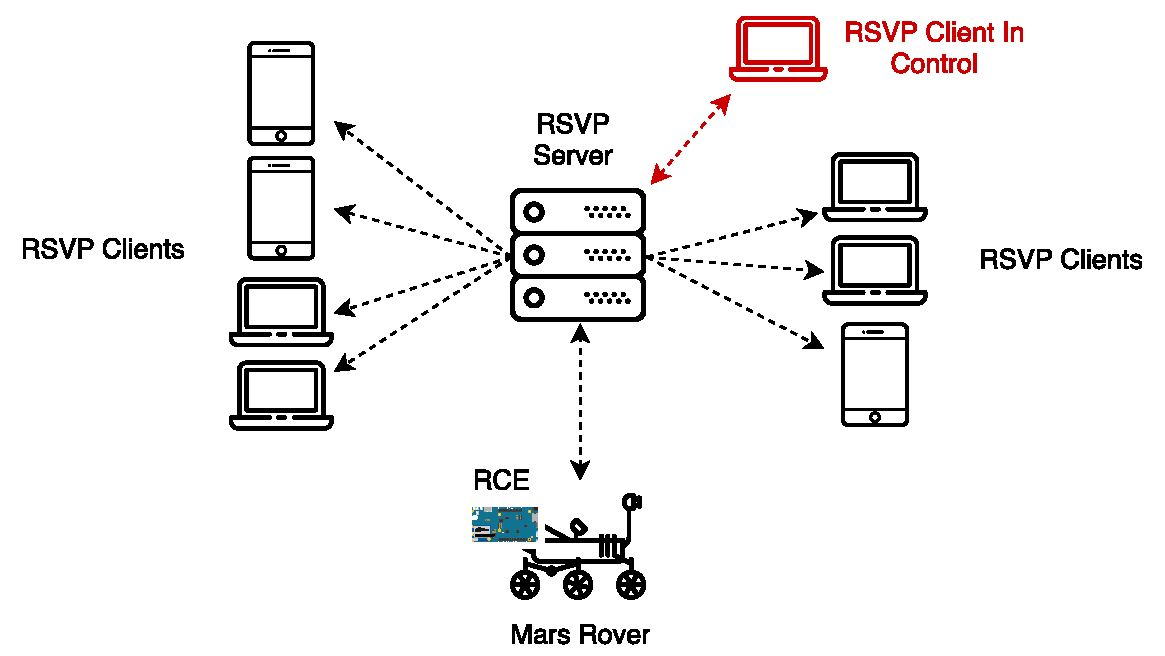
\includegraphics[width=0.7\linewidth]{figures/softDesign-useOverview}
      \caption[Diagramatic depiction of a typical use scenario of the software system]{Diagramatic depiction of a typical use scenario of the software system}
      \label{fig:softDesign-useOverview}
    \end{figure}

    An overview of the entire software system on a very high level is shown in Figure~\ref{fig:softDesign-useOverview}, a typical scenario involving the operational rover, the RSVP server in communication with the RCE and multiple RSVP Clients connected to the Server. The intention was to have the system be capable of allowing multiple devices on the network to connect to and interact with the system and one of the devices to have rover control access. The RSVP Server would manage the connected Clients and decide which of them would be able to control the rover. The principle behind the choice of which Client becomes the controlling Client is discussed later on.
    
  \subsection{Plan of Structure}
    In order to effectively coordinate the design and development of the software system as a whole, structural plans of the system and the subsystems within were constructed. The plans also aided the realisation of requirements and, further, choices of software technologies to use for each of the subsystems and components. The high level structure of the three subsystems and their interconnectedness was designed before constructing more detailed perspectives of each of them.
    
    \subsubsection{System Architectural Structure}            
      Figure~\ref{fig:softDesign-sysArchitectureStructure} is a high-level diagram showing a single-client scenario involving the three primary software subsystems and the means by which they were to communicate and interact. The solid arrows indicate wired connections and these exist on the RCE board for, as on the left, hardware communication and interfacing with sensory devices such as the camera. The RCE uses the wireless module to transmit video data and message data to the Server via the wireless module on the RCE board. The RSVP Server then offers the application source for the RSVP Client to be requested and loaded. Control, telemetry and video data is then sent and received between the RSVP Client and Server.

      \begin{figure}[h!]
        \centering
        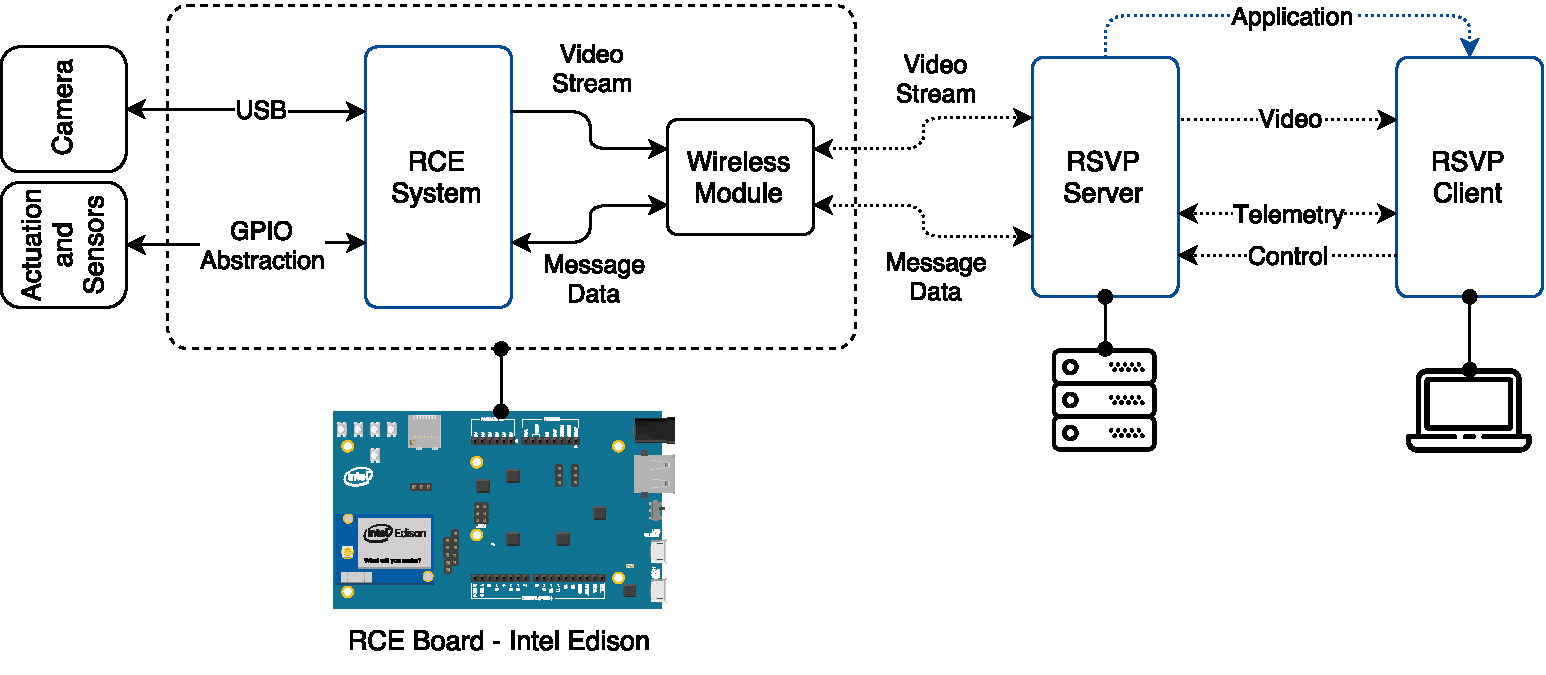
\includegraphics[width=1\linewidth]{figures/softDesign-sysArchitectureStructure}
        \caption[Diagram outlining the basic software system component structure]{Diagram outlining the basic software system component structure}
        \label{fig:softDesign-sysArchitectureStructure}
      \end{figure}
      
      As mentioned previously, the RSVP Server's primary role was to relay data between the RSVP Client and the RCE. Employing this structure for the flow of data allowed for many RSVP Client instances to exist and interface with the system. Not shown in Figure~\ref{fig:softDesign-sysArchitectureStructure} is the case where there are $N$ RSVP Clients on the network whereby one client would be in control of the rover, using the control, telemetry and video communication channels, and $N-1$ Clients would be receiving telemetry and video data only. Throughout the software design process, as much of the computational burden anticipated to exist in the system was offloaded onto the RSVP Server simply due to the fact that the RCE had the most severe computational performance limitations. The RSVP Server could be scaled to provide any required performance and thus could absorb functional components that were computationally taxing, an example of which is handling a large number of client connections that all require video and telemetry data. Communication specifics between all of the subsystems in Figure~\ref{fig:softDesign-sysArchitectureStructure} will be discussed in the design sections that follow as well as in the development sections.
      
      It can be seen in Figure~\ref{fig:softDesign-sysArchitectureStructure} that data transmission between all components of the system are grouped into two main channels: video data and message data. The separation of the two is made clearer in Section~\ref{subsubsec:rsvpServersPlan} which discusses the broadcast topology intended for use for the video data and how the data and the characteristics of the required communication naturally differ from that of telemetry and control data. Splitting of the two flows of data also allowed for finer control over the transmission in terms of setup sequences and during operation. As such, the message data channel between the Server and a Client was split on the basis of function.
      
  \subsection{Technology Choices}
    \subsubsection{Common Platform Flavour}
      The fact that the RCE board's computer supported the use of Linux as an operating system presented an opportunity to have all aspects of the software system follow suit in this regard, specifically the RSVP Server. The Server was intended to be flexible in form-factor to facilitate the open-sourcing secondary objective of the project and for the purpose of the system developed for this report, it was chosen to be a PC capable of running a distribution of Linux. Most distributions of Linux offer the stability and performance required by server-type processes and applications which explains the popularity of the operating system in network and internet service industries \cite{w3techs_Oct2016} and hence the decision to employ such as the operating system for the Server. The choice between heterogeneous and homogeneous architectures for the software system resolved to a trade-off between the advantage of technological flexibility as in the heterogeneous case and development simplicity in the other. Technological flexibility would have benefited the design in allowing choice of technologies that would better suit each of the subject components, perhaps to optimise resource consumption (storage, computation or even power) or improve compatibility with associated hardware and other components. Due to the limited time-frame of the project, the benefit of the ease of learning and design brought by a homogeneous system weighed in greater than flexibility, together with the abundance of packages and tools available for a Linux-based platform. Using Linux also supported the free, open-source software ideology making it more available to those who intend to be involved.
      
      \subheading{Javascript}\\\\
        With both the RCE and RSVP Server being based on a Linux platform as well as the RSVP Client being web-based (discussed further in Section~\ref{subsubsec:applicationFrontend}), another opportunity to employ a common technology across the system was presented, specifically the use of the Javascript language most commonly associated with websites and web applications. Using Javascript across the stack (including the RCE) followed the architecture pattern of homogeneity, simplified the learning process before development of the subsystems and minimised anticipated development overhead in terms software development environments and build tools. Using Javascript kept the project on a modern, popular and cutting edge trajectory and was a widely recognised full-stack solution used for services such as Netflix, Paypal, Medium, Uber, Twitter and Airbnb \cite{nodeusers_2016} \cite{driesbuytaert_2016}.
        
        A javascript runtime environment was required for the Server and RCE subsystems 
            
    \subsubsection{Embedded Software Platform}
    \subsubsection{The Web as an Application Front-end}
    \label{subsubsec:applicationFrontend}
    \subsubsection{Front-end Framework}
    \subsubsection{Message Data Communication}
    \subsubsection{Media Streaming}
    
  \subsection{Subsystem Design}
    \subsubsection{RCE Design}
      
    \subsubsection{RSVP Server Design}
    \label{subsubsec:rsvpServersPlan}
    \subsubsection{RSVP Client Design}
    
